\documentclass[a4paper,10pt]{article}
%\usepackage[latin1]{inputenc} % Paquetes de idioma
\usepackage[utf8]{inputenc} % Paquetes de idioma (Este encoding toma acentos :) )
\usepackage[spanish]{babel} % Paquetes de idioma
\usepackage{graphicx} % Paquete para ingresar gráficos
\usepackage{grffile}
\usepackage{hyperref}
\usepackage{fancybox}
\usepackage{amsmath}
\usepackage{amsfonts}
\usepackage{listings}
\usepackage{float}
% Paquetes de macros de Circuitos
%\usepackage{pstricks}
\usepackage{tikz}

% Encabezado y Pié de página
\usepackage{fancyhdr} % Paquete para encabezados y pie de página
\pagestyle{fancy} % Sin esta línea no se imprimiría el encabezado en todas las páginas

\fancyhf{} %  Borra el encabezado anterior (Por defecto escribe el títutlo de la sección en la que se encuentra la hoja
\setlength{\headheight}{22.55pt}
\fancyhead[L]{
	{\textsf{Facultad de Ingenier\'ia $-$ Universidad de Buenos Aires \\ 66.44 Instrumentos Electrónicos}}
}
%\addtocounter{page}{5}
\fancyhead[R]{\thepage}

\renewcommand{\footrulewidth}{0.4pt} % Ajusta el tamaño de las líneas separadoras en el pié de página
\renewcommand{\headrulewidth}{0.4pt} % Ajusta el tamaño de las líneas separadoras en el encabezado

\fancyfoot[L]{
	{\textsf{Trabajo Pr\'actico N$^{\circ}4$}: Mediciones de impedancias} \\
	{\textsf{Integrantes: Eduardo Sanchez, Francisco Soler}}
	}
		

% Carátula del Trabajo
\title{ \author{} % Lo pongo para que el warning no moleste :p
\setlength{\unitlength}{1cm} %  Especifica la unidad de trabajo
\thispagestyle{empty}

\begin{picture}(18,0)
\put(0,0){
\includegraphics[width=1.5cm, height=3cm]{Logo1.png}}

\put(10.5,0){
\includegraphics[width=3cm, height=3cm]{Logo2.png}}

\end{picture}
\\[1.5cm]
\begin{center}
	\textbf{{\Huge Facultad de Ingenier\'ia \\ Universidad de Buenos Aires}}\\[2cm]
	{66.44 Instrumentos Electrónicos}\\[0.5cm]
	{Trabajo Pr\'actico N$^{\circ}3$: Mediciones de impedancias}\\[2.5cm]
\end{center}

\begin{flushleft}
	\textbf{Integrantes:} \\[1cm]

	\begin{tabular}{|c|c|c|}
		\hline
		\textbf{\normalsize Padr\'on} & \textbf{\normalsize Nombre} & \textbf{\normalsize Email} \\
		\hline
		\normalsize 92903 & \normalsize Sanchez, Eduardo Hugo & \normalsize hugo\_044@hotmail.com \\
		\hline
		\normalsize 91227 & \normalsize Soler, Jos\'e Francisco & \normalsize francisco.\_tw@hotmail.com \\
		\hline
		\normalsize xxx & \normalsize Wawrynczak, Claudio  & \normalsize claudiozak@gmail.com \\
		\hline
	\end{tabular}
\end{flushleft}
\date{} % Hace que no se imprima la fecha en la cual se compilo el .tex
 }

\begin{document}
	\maketitle % Hace que el título anterior sea el principal del documento
	\newpage

	\tableofcontents % Esta línea genera un indice a partir de las secciones y 
					 % subsecciones creadas en el documento
	\newpage


	\section{Objetivo}
	
	\indent	El objetivo del presente trabajo práctico es determinar las 
	diferentes impedancias medidas utilizando un osciloscopio con técnicas de 
	reflectometría.
	
	\newpage
	\section{Desarrollo}
\indent Para llevar a cabo las mediciones, se utilizan los siguientes
		instrumentos:
		\begin{itemize}
			\item Un generador de pulsos Hewlett Packard 8082A.
			\item Un osciloscopio RIGOL DS1302CA ($BW=300MHz$).
			\item La punta Rigol RP3300.
			\item Cable coaxil para realizar las distintas conexiones entre 
			instrumentos.
		\end{itemize}	
	
		\subsection{Medici\'on 1- Velocidad de propagaci\'on de una l\'inea}
		\indent En esta medición se calcula el largo de distintos cables, para
		ello se conecta un generador y un osciloscopio en el mismo terminal 
		del cable por medio de un conector "T". El generador emite un pulso y,
		dependiendo que impedancia está conectada el otro terminal, la señal 
		rebota con la misma fase, fase opuesta o no se refleja absolutamente 
		nada. \\
		\indent Se mide el tiempo que tarda la señal en ir y volver por el 
		cable y, con dicho resultado, se calcula la velocidad de propagación 
		sobre el mismo.	\\
		\indent La imágenes \ref{a}, \ref{b} y \ref{c} muestran tres tipos de
		adaptaciones: izquierda posee un circuito abierto; medio, adaptado;
		derecha, cortocircuito. \\
	
			\begin{figure}[!htb]
				\centering
				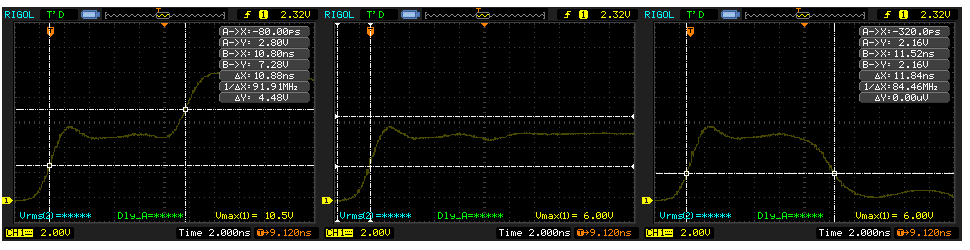
\includegraphics[width=9cm]
				{Imagenes/CableF&G.png}
				\caption{Propagación de la señal en un cable $RG-213/U$}
				\label{a}
			\end{figure}
			\begin{figure}[!htb]
				\centering
				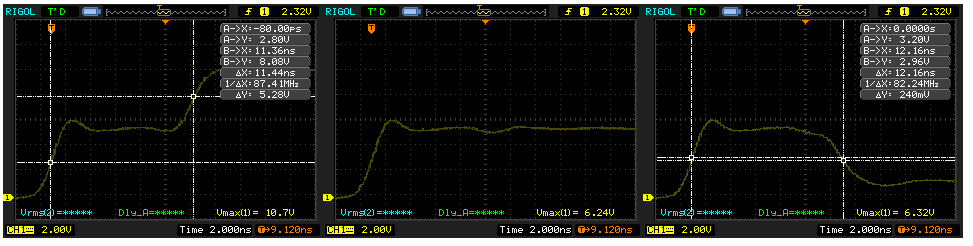
\includegraphics[width=9cm]
				{Imagenes/CableCoaxialFino.png}
				\caption{Propagación de la señal en un cable coaxial fino}
				\label{b}
			\end{figure}
			\begin{figure}[!htb]
				\centering
				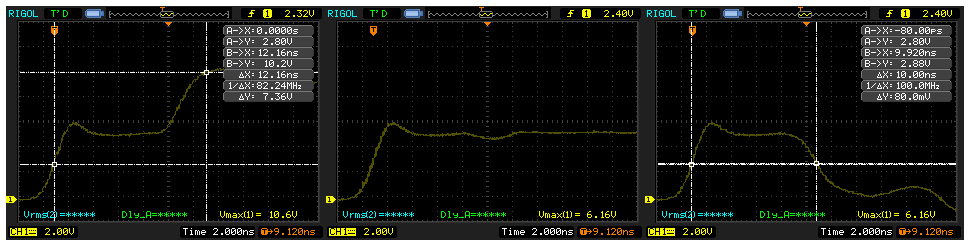
\includegraphics[width=9cm]
				{Imagenes/CableCoaxialGrueso.png}
				\caption{Propagación de la señal en un cable coaxial grueso}
				\label{c}
			\end{figure}
	
		\indent La tabla \ref{tab002} muestra los distintos cables con sus 
		respectivas longitudes (medidas con un metro), tiempo (medido en el 
		osciloscopio) y velocidad de propagación (calculada en base a los 
		anteriores resultados). En la longitud se está tomando en cuenta el 
		largo de la $T$ utilizada para conectar el osciloscopio al cable, el 
		cual mide $18 cm$ (su incerteza se incluye en los $\pm2\text{cm}$ de 
		la medici\'on total que se ha tomado para todas las mediciones). \\
		
		\begin{table}[!htp]
			\centering
			\begin{tabular}{|c|c|c|c|}
				\hline
	    		Cable & longitud total & $\tau$ & Vel propagación \\
				\hline
				F\&G RG-213/u & $118~\text{cm}~\pm2\text{cm} $ & 
				$10.88~\mu\text{n seg}~\pm0,62\text{nseg}$ & 
				$(0.36~\pm0.006)~\cdot\text{c}$ \\
				\hline 
				coaxil fino & $124~\text{cm}~\pm2\text{cm}$ & 
				$11.44~\mu\text{n seg}~\pm0,62\text{nseg}$ &
				$(0.36~\pm0.006)~\cdot\text{c}$ \\
				\hline
				coaxil grueso & $144~\text{cm}~\pm2\text{cm}$ & 
				$12.16~\mu\text{n seg}~\pm0,62\text{nseg}$ & 
				$(0.39~\pm0.005)~\cdot\text{c}$ \\
				\hline
			\end{tabular}
			\caption{Comparación de velocidades de propagación entre distintos 
			tipos de cables} \label{tab001}
		\end{table}	
	 Como se puede apreciar, la velocidad de propagaci\'on se obtiene con baja
	 incerteza, con lo cual el m\'etodo aplicado resulta \'util para este fin.

	\subsection{Medición 2 - Resistencias}
	\indent En esta sección se pretende conocer el valor de diferentes 
	resistencias por medio de reflectometr\'ia. Por otra parte tambi\'en se 
	desea conocer la exactitud del m\'etodo para obtener impedancias. Por ello
	se dispone de 5 resistores, de resistencias conocidas para contrastar su 
	valor. \\
	\indent El banco de medición consiste en el osciloscopio conectado con una
	T, con un extremo conectado a un generador de pulsos y otro extremo 
	conectado a un cable coaxil, el cual a su vez en su extremo est\'a 
	conectado a alguna de las resistencias. La idea consiste en observar el 
	coeficiente de reflexión, $\rho$, de la l\'inea de transmisión y con \'el,
	la carga de la l\'inea aplicando la siguiente relaci\'on: 
	$$\rho=\frac{Z_L-Z_0}{Z_L+Z_0}$$
	
	\indent En la Figura \ref{img001} se muestra el resultado obtenido cuando 
	se carg\'o el cable coaxil con la resistencia de $10k\Omega$. Puede verse 
	que $$\rho=\frac{Z_L-Z_0}{Z_L+Z_0}$$
	$$\frac{3.24V}{3.40V}=\frac{Z_L- 50\Omega}{Z_L+50\Omega}$$
	$$(Z_L+50\Omega) \cdot \frac{3.24V}{3.40V}=Z_L- 50\Omega$$
	$$Z_L = 50\Omega\cdot\frac{1 + \frac{3.24V}{3.40V}}{1-\frac{3.24V}{3.40V}}
	= 2075\Omega$$
	
	\indent En general, la siguiente relaci\'on puede deducirse, despejando 
	$Z_L$ en funci\'on de $\rho$ 
	$$Z_L = Z_0\cdot\frac{1 + \rho}{1-\rho} $$

	\indent Para propagar errores se parte calculando la incertidumbre que 
	posee la medición de $V+$ y $V-$ las cuales son obtenidas directamente de 
	las incertidumbres del osciloscopio. De la hoja de datos del fabricante, 
	se obtiene que la incertidumbre vertical de una medici\'on (para la 
	resoluci\'on utilizada de $1V/div$) es del $3\%$. Con lo cual la incerteza
	relativa de $\rho=\frac{V+}{V-}$ es del $6\%$ ya que como se demuestra a 
	continuaci\'on en la divisi'on las incertezas relativas se suman.
	
	\indent Primero se procede a calcular la incertidumbre de $\rho$, la cual
	se obtiene de la siguiente forma
	
	$$\rho = \frac{V+}{V-} \pm \Delta\rho$$
	$$\Delta\rho = (\epsilon_{V+} + \epsilon_{V-})\cdot\rho$$

	\indent Una vez obtenido $\rho$, se procede a calcular cada parte de la 
	división, se sabe que la incertidumbre absoluta es la misma cuando se suma o
	resta por una constante, y se sabe que la incertidumbre relativa de la 
	división o multiplicación es igual a la suma de las incertidumbres relativas
	de cada variable.

	$$1 + \rho = (1 + \rho) \pm \Delta\rho$$
	$$1 - \rho = (1 - \rho) \pm \Delta\rho$$
	$$\epsilon_{\frac{1 + \rho}{1 - \rho}} = \epsilon_{1 + \rho} + 
	\epsilon_{1 - \rho}$$

	$$\epsilon_{\frac{1 + \rho}{1 - \rho}} = \frac{\Delta\rho}{1 + \rho} + 
	\frac{\Delta\rho}{1 - \rho}$$
	$$\epsilon_{\frac{1 + \rho}{1 - \rho}} = \frac{2\cdot\Delta\rho}
	{1 - \rho^2}$$
	
	\indent Ahora se procederá a calcular la incertidumbre absoluta de la 
	división

	$$\Delta_{\frac{1 + \rho}{1 - \rho}} = \epsilon_{\frac{1 + \rho}{1 - \rho}}
	\cdot\frac{1+\rho}{1 - \rho}$$
	
	$$\Delta_{\frac{1 + \rho}{1 - \rho}} = \frac{2\cdot\Delta\rho}{(1 - \rho)^2}
	$$
	\indent Por último solo queda determinar la incertidumbre absoluta de $Z_L$,
	la cual, es la calculada anteriormente, pero escalada por $Z_0$ resultando:

	$$\Delta_{Z_L} = Z_0\cdot\Delta\frac{1 + \rho}{1 - \rho}$$
	$$\Delta_{Z_L} = Z_0\cdot\frac{2\cdot\Delta\rho}{(1 - \rho)^2}$$

	\indent De esta forma, queda determinada $Z_L$

	$$Z_L =Z_0\cdot\frac{1+\rho}{1-\rho} \pm Z_0\cdot\frac{2\cdot\Delta\rho}
	{(1 - \rho)^2}$$

	\indent Por lo tanto $Z_L=2k\Omega~\pm~2,5k\Omega$, el cual no es un valor
	cercano a los $10k\Omega$  esperados. De hecho su incerteza es del mismo 
	orden que el valor de referencia, con lo cual se concluye que no es una 
	buena medici\'on y deber\'a encontrarse otro m\'etodo para hallar con 
	mayor precisi\'on su valor.\\
		
		\begin{figure}[!htb]
			\centering
			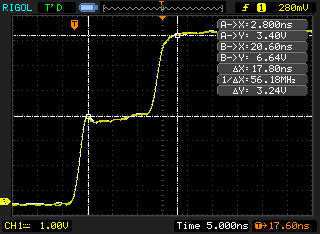
\includegraphics[width=8cm]
			{Imagenes/Res10k.png}
			\caption{Medici\'on para la resistencia de $10k\Omega$. La 
			referencia (en blanco) esta graficada con la l\'inea abierta.}
			\label{img001} 
		\end{figure}

	\indent En la Figura \ref{img002} se muestra el resultado con la 
	resistencia de $1k\Omega$. Puede verse que 
	$$\rho=\frac{Z_L-Z_0}{Z_L+Z_0}$$
	$$\frac{2.96V}{3.40V}=\frac{Z_L- 50\Omega}{Z_L+50\Omega}$$
	
	\indent Por lo tanto $Z_L=722\Omega~\pm~311\Omega$, que se corresponde a 
	un valor, si bien aun lejano, m\'as pr\'oximo que en el caso anterior, 
	pero con una incerteza considerable.
		
		\begin{figure}[!htb]
			\centering
			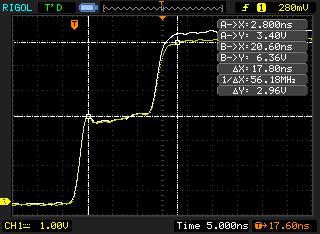
\includegraphics[width=8cm]
			{Imagenes/Res1k.png}
			\caption{Medici\'on para la resistencia de $1k\Omega$. La 
			referencia (en blanco) esta graficada con la l\'inea abierta.}
			\label{img002} 
		\end{figure}

	\indent En la Figura \ref{img003} se muestra el resultado con la 
	resistencia de $120\Omega$. Puede verse que 
	$$\rho=\frac{Z_L-Z_0}{Z_L+Z_0}$$
	$$\frac{1.44V}{3.40V}=\frac{Z_L- 50\Omega}{Z_L+50\Omega}$$
	
	\indent Por lo tanto $Z_L=123\Omega~\pm~7.6\Omega$, el cual es un valor 
	que se encuentra dentro de la tolerancia de la resistencia ($120\Omega 
	\pm 10\%$ para resistores de carb\'on). 	

		\begin{figure}[!htb]
			\centering
			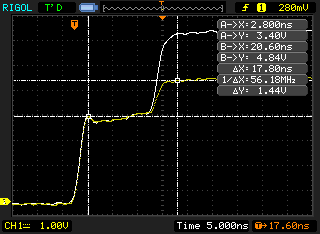
\includegraphics[width=8cm]
			{Imagenes/Res120.png}
			\caption{Medici\'on para la resistencia de $120\Omega$. La 
			referencia (en blanco) esta graficada con la l\'inea abierta.}
			\label{img003}
		\end{figure}
	
	\indent En la Figura \ref{img004} se muestra el resultado con la 
	resistencia de $47\Omega$. Dado su valor cercano a la impedancia 
	caracter\'istica, como era de esperar la onda reflejada es peque\~na. Como
	antes, $$\rho=\frac{Z_L-Z_0}{Z_L+Z_0}$$
	$$\frac{-120mV}{3.48V}=\frac{Z_L- 50\Omega}{Z_L+50\Omega}$$
	\indent Despejando, se obtiene $Z_L=46.6\Omega~\pm~0.2\Omega$, 
	pr\'acticamente coincidiendo con el valor de referencia de $47\Omega$. 
	Debe notarse tambi\'en que la incerteza obtenida es muy peque\~na y 
	\'esta fue reduciendose a medida que el coeficiente de reflexi\'on 
	disminu\'ia de $1$ (valor donde te\'oricamente la incertidumbre es 
	infinita seg\'un la expresi\'on desarrollada 
	$Z_0\cdot\frac{2\cdot\Delta\rho}{(1 - \rho)^2}$)
	
		\begin{figure}[!htb]
			\centering
			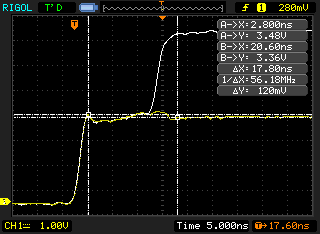
\includegraphics[width=8cm]
			{Imagenes/Res47.png}
			\caption{Medici\'on para la resistencia de $47\Omega$. La 
			referencia (en blanco) esta graficada con la l\'inea abierta.}
			\label{img004}
		\end{figure}

	\indent Por \'ultimo en la Figura \ref{img005}, se realiza la medici\'on 
	con la resistencia de $3.90\Omega$. Como se puede apreciar es un valor 
	pr\'oximo a un cortocircuito, con lo cual en el gr\'afico se puede 
	observar que el pulso se recorta. Como $$\rho=\frac{Z_L-Z_0}{Z_L+Z_0}$$
	$$\frac{-2.60V}{3.44V}=\frac{Z_L- 50\Omega}{Z_L+50\Omega}$$
	
	\indent Con lo cual $Z_L=6.9\Omega~\pm~1.50\Omega$ y se aleja del un poco 
	del valor $3.9\Omega$ de referencia
		
		\begin{figure}[!htb]
			\centering
			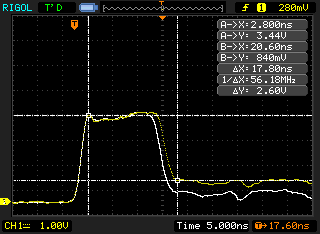
\includegraphics[width=8cm]
			{Imagenes/Res3e9.png}
			\caption{Medici\'on para la resistencia de $3.9\Omega$. La 
			referencia (en blanco) esta graficada con la l\'inea en 
			cortocircuito.}
			\label{img005}
		\end{figure}

	\indent Cabe destacar las irregularidades que se observan en la parte 
	horizontal de la señal, esto se puede atribuir a la línea de transmisión,
	dado que, si el cable tiene golpes, torceduras, desperfectos, presentará 
	cambios de impedancias donde están dichos desperfectos. Esto genera que 
	haya señales reflejadas a lo largo de la línea, pero de una amplitud muy 
	pequeña, como cada una se refleja en una posición del calbe distinta, 
	llegan al osciloscopio a distintos tiempos. Observándose así dichas 
	irregularidades. Otro causante puede ser una desadaptación del 
	osciloscopio a la línea, la cual también generaría una onda estacionaria 
	que se va atenuando en cada cambio de impedancia.

	\indent De los resultados obtenidos, cuyo resumen se muestra en la Tabla 
	\ref{tab001}, debe notarse que las mediciones de menor incertidumbre son 
	aquellas cuya resistencia de carga es cercana a la impedancia 
	caracter\'istica. En particular las resistencias mucho mayores a $Z_0$, como
	la de $10k\Omega$ tienen una incertidumbre elevada y esto se debe a que para
	$0\leq \rho \leq 1$ est\'an asociadas resistencias del orden 
	$Z_0 \leq R_L \leq \infty$, con lo cual la exactitud es menor. Diferente 
	es el caso cuando $-1\leq \rho \leq 0$ que se asocia a resistencias 
	comprendidas en $0\Omega \leq R_L \leq Z_0$, con lo cual la exactitud es 
	mayor en estos casos.

	
		\begin{table}[!htp]
			\centering
			\begin{tabular}{|c|c|c|c|}
				\hline
    			Valor de referencia & Medici\'on & Variaci\'on respecto de la
				referencia \\
				\hline
				$10k\Omega$ & $2k\Omega~\pm~2,5k\Omega$ &$-80 \% $ \\
				\hline 
				$1k\Omega$ & $722\Omega~\pm~311\Omega$ &$-27.8\%$\\
				\hline
				$120\Omega$ & $123\Omega~\pm~7.6\Omega$ &$2.5\% $ \\
				\hline
				$47\Omega$ & $46.6\Omega~\pm~0.2\Omega$ &$0.85\% $ \\
				\hline
				$3.9\Omega$ & $6.9\Omega~\pm~1.5\Omega$ &$76\% $  \\
				\hline								
			\end{tabular}
			\caption{Resumen de los resultados obtenidos para las resistencias
			} 
			\label{tab001}
		\end{table}
		
						
	\subsection{Medición 3 - Bobina}
	\indent En esta secci\'on se pretende medir la inductancia de una bobina y
	su valor de resistencia equivalente serie. El banco de medici\'on es el 
	mismo que el anterior solo que la l\'inea se carga con el inductor. \\
	\indent Cuando el flanco del pulso incidente llegue al inductor, este 
	presentar\'a alta impedancia, con lo cual, inicialmente la respuesta se 
	asemeja a aquella en la que la l\'inea est\'a abierta. La respuesta 
	decaer\'a exponencialmente con $\tau=\frac{L}{Z_0+R_L}$, donde $R_L$ es la
	resistencia serie del inductor, hasta un valor de tensi\'on no nulo que 
	permite conocer el valor de $R_L$ por medio del coeficiente de 
	reflexi\'on. \\
	\indent En la Figura \ref{img006}, se puede observar la respuesta temporal
	cuando se carga la l\'inea con el inductor. Como se esperaba la respuesta
	es exponencial decreciente con 
	$\tau=\frac{L}{Z_0+R_L}=580ns\pm 0.6ns$, como $Z_0=50\Omega$ es 
	necesario conocer el valor de $R_L$, para saber el de $L$. Despejando L y
	propagando incertezas se obtiene
	$$L=\tau(Z_0+R_L)\pm ( (Z_0+R_L)\Delta\tau+\tau\Delta R_L)$$
		
		\begin{figure}[!htb]
			\centering
			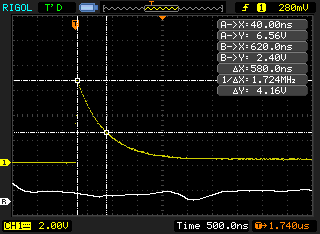
\includegraphics[width=8cm]
			{Imagenes/InductorL.png}
			\caption{Respuesta temporal para la medici\'on de la inductancia 
			de una bobina.}
			\label{img006}
		\end{figure}

	\indent De la Figura \ref{img007} puede hallarse el valor residual de 
	tensi\'on y aplicar la relaci\'on  $\rho=\frac{R_L-Z_0}{R_L+Z_0}$, para 
	obtener la resistencia serie del inductor. De esta manera 
	$$\frac{320mV-3.40V}{3.40V}=\frac{R_L-50\Omega}{R_L-50\Omega}$$
	
	\indent Con lo cual $R_L=2.5\Omega~\pm 1.5\Omega$ y por lo tanto 
	$L=30,45\mu Hy~\pm 900nHy$ (una incerteza relativa del $2.95\%$), el 
	valor que difiere solamente un $1.5\% $ del valor de referencia (
	$L_{ref}=30\mu Hy$). Con lo cual se concluye que resulta un buen m\'etodo
	para medir la inductancia de una bobina, no as\'i para conocer su 
	resistencia serie equivalente, cuya incerteza relativa es del $60 \%$
	
		\begin{figure}[!htb]
			\centering
			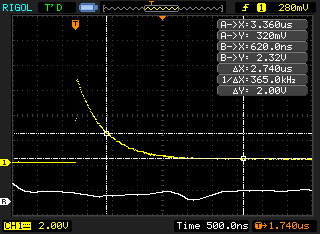
\includegraphics[width=8cm]
			{Imagenes/InductorR.png}
			\caption{Respuesta temporal para la medici\'on de la resistencia 
			equivalente serie de una bobina.}
			\label{img007}
		\end{figure}			
	
	
	\subsection{Medición 4 - Cortocircuito}
	\indent En esta medici\'on se coloca en el extremo de la l\'inea de 
	transmisi\'on un conductor. Idealmente esto generar\'ia una onda reflejada
	de la misma amplitud pero en contrafase respecto a la incidente (es decir,
	$\rho=-1$). Sin embargo, de la Figura \ref{img008} puede observarse un 
	sobrepico similar al hallado en la secci\'on anterior. Con lo cual se 
	concluye que ese conductor tiene una componente inductiva que se procede a
	estimar. \\
	\indent Dado que $\tau=\frac{L}{Z_0+R_c}=6ns~\pm~0.6ns$,  $Z_0=50\Omega$ y 
	$R_c\approx 0\Omega$, entonces
	$$L=\tau Z_0~\pm~Z_0\Delta\tau$$
	$$L=6ns 50\Omega~\pm~50\Omega0.6ns=300nHy~\pm~30nHy$$
	
	\indent La incerteza relativa es del $10 \%$, con lo cual se considera que
	es una medici\'on v\'alida pero resulta conveniente utilizar otro m\'etodo
	o bien otro instrumento para caracterizar mejor la inductancia equivalente
	del cortocircuito.

		\begin{figure}[!htb]
			\centering
			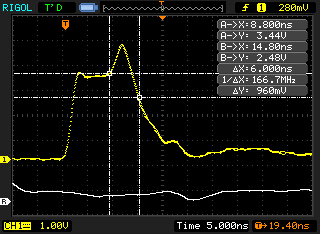
\includegraphics[width=8cm]
			{Imagenes/CORTO.png}
			\caption{Respuesta temporal para la medici\'on de la inductancia 
			equivalente de un conductor.}
			\label{img008}
		\end{figure}
		
	\subsection{Medición 5 - Capacitor}
	\indent En esta medición se utilizaron 3 capacitores distintos para medir
	la resistencia y capacidad equivalente. Los valores utilizados fueron 
	$100pF$, $180pF$ y $47nF$ (todos con una tolerancia del $20\%$) \\
	\indent La imagen \ref{img010} muestra las respuestas de dichas 
	mediciones. La figura de la izquierda es la respuesta del capacitor de 
	$100pF$, la del medio posee uno de $180pF$ y la de la derecha $47nF$. \\
	
		\begin{figure}[!htb]
			\centering
			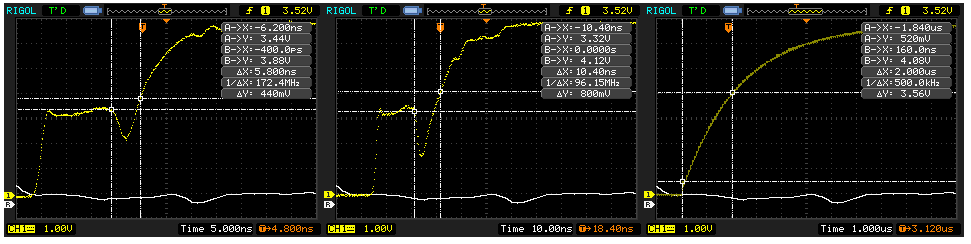
\includegraphics[width=12cm]
			{Imagenes/CurvasCapacitor.png}
			\caption{Respuestas de los distintos capacitores}
			\label{img010} 
		\end{figure}

	\indent Para poder determinar el capacitor y resitencia equivalente lo 
	primero que se hace es determinar el tiempo de crecimiento $\tau$. El cual
	posee la siguiente fórmula

		\begin{equation}
			\tau = R\cdot C
		\end{equation}
	
	\indent La línea de transmisión posee una impedancia característica de 
	$50\Omega$. Se desprecia la resistencia interna del capacitor. \\
	\indent Despejando el valor de C, en la tabla \ref{tab002} se reflejan los 
	resultados calculados con su respectivas incertidumbres. La expresi\'on 
	para obtener C con su incerteza es la siguiente
		\begin{equation}
			C = \frac{\tau}{R}\pm \frac{\Delta\tau}{R}
		\end{equation}
	\indent La incertidumbre de la medición del $\tau$ viene dada por el 
	osciloscopio, el cual posee la siguiente incertidumbre
		
		$$\Delta\tau = \frac{1}{2}~\text{nSec} + 50~\text{ppm}\cdot
		~\text{reading} + 0.6~\text{Seg}$$

		\begin{table}[!htp]
			\centering
			\begin{tabular}{|c|c|c|c|c|}
				\hline
    			C teórico & $\tau$ medido & $\Delta\tau$ & 
				C medido & $\Delta$C \\
				\hline
				100 pF & $5.8~\text{n seg}$ & $1.1~\text{n seg}$ & 
				116~\text{pF} & 22~\text{pF} \\
				\hline 
				180 pF & $10.4~\text{n seg}$ & $1.1~\text{n seg}$ &
				208~\text{pF} & 22~\text{pF} \\
				\hline
				47 nF & $2~\mu\text{seg}$ & $1.2~\text{n seg}$ & 40~\text{nF}
				& 24~\text{pF} \\
				\hline
			\end{tabular}
			\caption{Capacitancias medidas} 
			\label{tab002} 
		\end{table}

	\indent Se puede observar que este método sirve para medir capacitores 
	de magnitudes superiores a los $200pF$, dado que la incertidumbre relativa
	de dicha medición ronda los $12\%$.
	\newpage
	\section{Conclusiones}
	\indent La reflectometría, a partir de los resultados obtenidos, resulta 
	adecuada para realizar mediciones de velocidad de propagaci\'on con baja 
	incertidumbre (menor al $2 \%$ en el peor caso).\\
	\indent De las mediciones de resistencias utilizando reflectometría cabe 
	destacar que el valor medidio posee más incertidumbre a medida que el 
	valor de resistencia se aleja de la impedancia característica de la línea.
	Con lo cual deber\'a considerarse utilizar otro m\'etodo para caracterizar
	estas resistencias de valores mayores a la impedancia caracter\'istica del
	cable.	\\
	\indent Para las mediciones tanto de inductacias como de capacitancias 
	cabe destacar que, como se están midiendo tiempos de crecimiento, y 
	mientras se	asuma que la línea es sin pérdidas, las incertidumbres de 
	medición solo dependen del osciloscopio, por lo tanto, no varía en base al
	valor de capacidad a medir.\\
\end{document}

